
%%%%%%%%%%%%%%%%%%%%%%% file typeinst.tex %%%%%%%%%%%%%%%%%%%%%%%%%
%
% This is the LaTeX source for the TDPTemplate using
% the LaTeX document class 'llncs.cls' Springer LNAI format
% used in the RoboCup Symposium submissions.
% http://www.springer.com/computer/lncs?SGWID=0-164-6-793341-0
%
% It may be used as a template for your own TDP - copy it
% to a new file with a new name and use it as the basis
% for your Team Description Paper
%
% NB: the document class 'llncs' has its own and detailed documentation, see
% ftp://ftp.springer.de/data/pubftp/pub/tex/latex/llncs/latex2e/llncsdoc.pdf
%
%%%%%%%%%%%%%%%%%%%%%%%%%%%%%%%%%%%%%%%%%%%%%%%%%%%%%%%%%%%%%%%%%%%

\documentclass[runningheads,a4paper]{llncs}

% document input
\usepackage[utf8]{inputenc}		% input encoding
\usepackage[english]{babel}		% input language for hyphens

% fonts
\usepackage[T1]{fontenc}		% more glyphs and a
\usepackage{lmodern}			% better looking font

% page geometry
%\usepackage{a4wide}
%\usepackage{a4}
%\usepackage[left=48mm,right=46mm]{geometry}
\usepackage[left=32mm,right=31mm]{geometry}

\usepackage{amssymb}
\usepackage{amsmath}
\setcounter{tocdepth}{3}


\usepackage{hyperref}
\usepackage{graphicx}
\usepackage{caption}
\usepackage{subcaption}
\captionsetup{compatibility=false}
\usepackage{float}

\usepackage{url}
\usepackage{listings}

% *** MORE GRAHPICS ***
\usepackage[usenames,dvipsnames]{color}

% *** BIBLIOGRAPHY PACKAGES ***
%\usepackage{natbib}

%%%%%%%%%%%%%%%%%%%%%%%%%%%%%%%%%%%%%%%%%%%%%%%%%%%%%%%%%%%%%%%%%%%
\usepackage{booktabs}           % For tables (toprule, midrule, bottomrule)
\usepackage{todonotes}			% should be defined after the color package
%%%%%%%%%%%%%%%%%%%%%%%%%%%%%%%%%%%%%%%%%%%%%%%%%%%%%%%%%%%%%%%%%%%

%%%%%%%%%%%%%%%%%%%%%%%%%%%%%%%%%%%%%%%%%%%%%%%%%%%%%%%%%%%%%%%%%%%
% *** PATHS ***
\makeatletter
\def\input@path{{Figures/}		
				}
\makeatother

\graphicspath{  {Figures/}
				}
%%%%%%%%%%%%%%%%%%%%%%%%%%%%%%%%%%%%%%%%%%%%%%%%%%%%%%%%%%%%%%%%%%%

%%%%%%%%%%%%%%%%%%%%%%%%%%%%%%%%%%%%%%%%%%%%%%%%%%%%%%%%%%%%%%%%%%%

% Acronym definitions
\usepackage[acronym]{glossaries}
\newacronym{ed}{ED}{Environment Descriptor}
\newacronym{amcl}{AMCL}{Adaptive Monte Carlo Localization}
\newacronym{gui}{GUI}{Graphical User Interface}
\newacronym{spl}{SPL}{Standard Platform League}
\newacronym{fcfg}{FCFG}{feature context free grammar}
\newacronym{ros}{ROS}{Robot Operating System}
\newacronym{wire}{WIRE}{World Information for Robotic Environments}
\newacronym{cnn}{CNN}{Convolution Neural Networks}

% shorthand definitions
\newcommand{\eg}{\emph{e.g.}}						% Exemplum gratia
\newcommand{\goal}{\mathcal{G}}						% Goal area
\newcommand{\goallc}{\mathcal{G}_{\mathrm{lc}}}		% Subset of goal area with costs below threshold cmin
\newcommand{\goalhc}{\mathcal{G}_{\mathrm{hc}}}		% Subset of goal area with costs above threshold cmin
\newcommand{\ie}{\emph{i.e.}}						% Id est
%%%%%%%%%%%%%%%%%%%%%%%%%%%%%%%%%%%%%%%%%%%%%%%%%%%%%%%%%%%%%%%%%%%

\begin{document}

\title{Tech United Eindhoven @Home \acrshort{spl}\\2017 Team Description Paper}
\author{M.F.B.~van~der~Burgh, J.J.M.~Lunenburg, R.P.W.~Appeldoorn, R.W.J.~Wijnands, T.T.G.~Clephas, M.J.J.~Baeten, L.L.A.M.~van~Beek, R.A.~Ottervanger, H.W.A.M~van~Rooy, J.~Scholtes and M.J.G.~van~de~Molengraft}
\institute{Eindhoven University of Technology,
\newline Den Dolech 2, P.O. Box 513, 5600 MB Eindhoven, The Netherlands\\
\texttt{http://www.techunited.nl, techunited@tue.nl, https://github.com/tue-robotics}}
\authorrunning{Tech United Eindhoven}

%\author{Team Leader \and Team Members }
%\institute{[Intitute name and direction here], \\
%\texttt{http://devoted-web-site.url}}
\maketitle


%%%%%%%%%%%%%%%%%%%%%%%%%%%%%%%%%%%%%%%%%%%%%%%%%%%%%%%%%%%%%%%%%%%%%%%%%%%%%%%%%%%%

\begin{abstract}
This paper describes the research interest and technical approach of the Tech United team towards using the Toyota HSR system for the RoboCup @HOME standard league. Tech United will use an advanced world modelling representation system called the Environment Descriptor (open source) that allows straight forward implementation of localization, navigation, exploration, object detection \& recognition, object manipulation and robot-robot cooperation skills. This will yield a fast development to create added functionality for the HSR system and to be used by the open source community. Recently developments are improved object detection via deep learning methods, a generic GUI for different user levels and improved natural language interpretation.
\end{abstract}

%%%%%%%%%%%%%%%%%%%%%%%%%%%%%%%%%%%%%%%%%%%%%%%%%%%%%%%%%%%%%%%%%%%%%%%%%%%%%%%%%%%%

\section{Introduction}
Tech United Eindhoven is the RoboCup student team of Eindhoven University of Technology that (since 2005) successfully competes in the robot soccer Middle Size League (MSL) and later (2011) joined the ambitious @Home League. The Tech United @Home team currently holds the runner up title of RoboCup 2016 in Leipzig and is the reigning European Champion. (2016 RoboCup European Open, Eindhoven)

Our ambition is to extend our team, efforts and expertise with a new winner: the Toyota Human Support Robot (HSR). This standard platform will enable us to further increase our impact on the robotics open source community.

We are driven by our personal believe that service robots will have an immensely positive impact on the quality of live and independence of people; especially elderly and physically impaired people can benefit from this ground-breaking technology. It is not only valuable technology, but also has urgency as most of the western economies have an aging society. We are therefore intrinsically motivated to contribute to the open source community to move this technology to new boundaries that allow robots to safely, robustly and effectively function and work around people. 

It is our firm believe that the impact, acceptance and use of new technology greatly depends on standardization of hardware and software systems. Metaphorically this is the foundation upon which great technology can be build and scaled. We see the availability of the HSR as a step forward in creating an eco-system that fosters new innovation and pushed the boundaries of what’s possible. 

This proposal will explain our development plans with the Toyota HSR system.

%\newpage
\section{Description of the approach planned to be implemented on the robot}
This section will explain the methods and software that will be used to solve the RoboCup@Home challenges with the Toyota HSR system.

\subsection{\acrfull{ed}}
The TUe \acrfull{ed} is a \acrfull{ros} based 3D geometric, object-based world representation system for robots. In itself ED is database system that structures multi-modal sensor information and represents this in an object-based world representation that can be utilized for robot localisation, navigation, manipulation and interaction functions. See Figure \ref{fig:ed} for a schematic overview of \href{https://github.com/tue-robotics/ed}{ED}. %\footnote{\acrshort{ed} is an evolution of \acrfull{wire}, that was created in the FP7 RoboEarth Project. Secondly, ED is utilized within the RoboCup @home competition (also read the \href{https://github.com/tue-robotics/team_description_paper/blob/master/Tech_United_At_Home_TDP_2015.pdf}{TU/e 2015 TDP} for RoboCup). More information, software, installation manual and tutorial can be found on \url{https://github.com/tue-robotics/ed}}
%An elaborate explanation, including tutorials are available at our GitHub website \footnote{\url{http://github.com/tue-robotics}}.
Tech United uses ED in its AMIGO and SERGIO robots that participate (and collaborate) in the @Home league. In previous years, developments have been focussed towards making ED platform independent. As a results ED had been used on the PR2 system, Turtlebot and Dr. Robot systems (X80).
\begin{figure}[h]
    %\vspace{-0.3cm}
	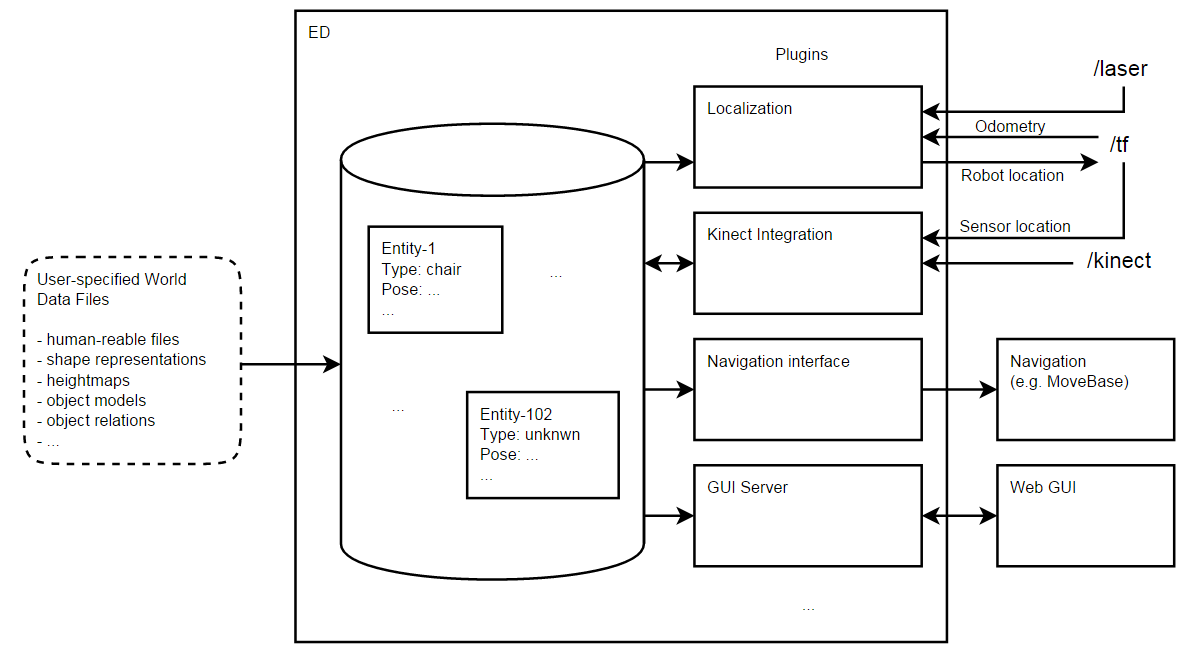
\includegraphics[width = \linewidth]{Figures/ed_overview}
    %\vspace{-1em}
	\caption{schematic overview of TUe Environment Descriptor.}
	\label{fig:ed}
    %\vspace{-0.5cm}
\end{figure}
ED is one re-usable environment description that can be used for a multitude of needed functionalities. Instead of having different environment representations for localization \acrfull{amcl}, navigation (MoveBase), manipulation (MoveIt!), interaction, etc.. An improvement in this single, central world model will reflect in the performances of the separate robot capabilities. It omits updating and synchronization of multiple world models. At the moment different ED modules exist which enable robots to localize themselves, update positions of known objects based on recent sensor data, segment and store newly encountered objects and visualize all this through a web-based \acrshort{gui}.
\begin{figure}[h]
\centering
    %\vspace{-0.3cm}
	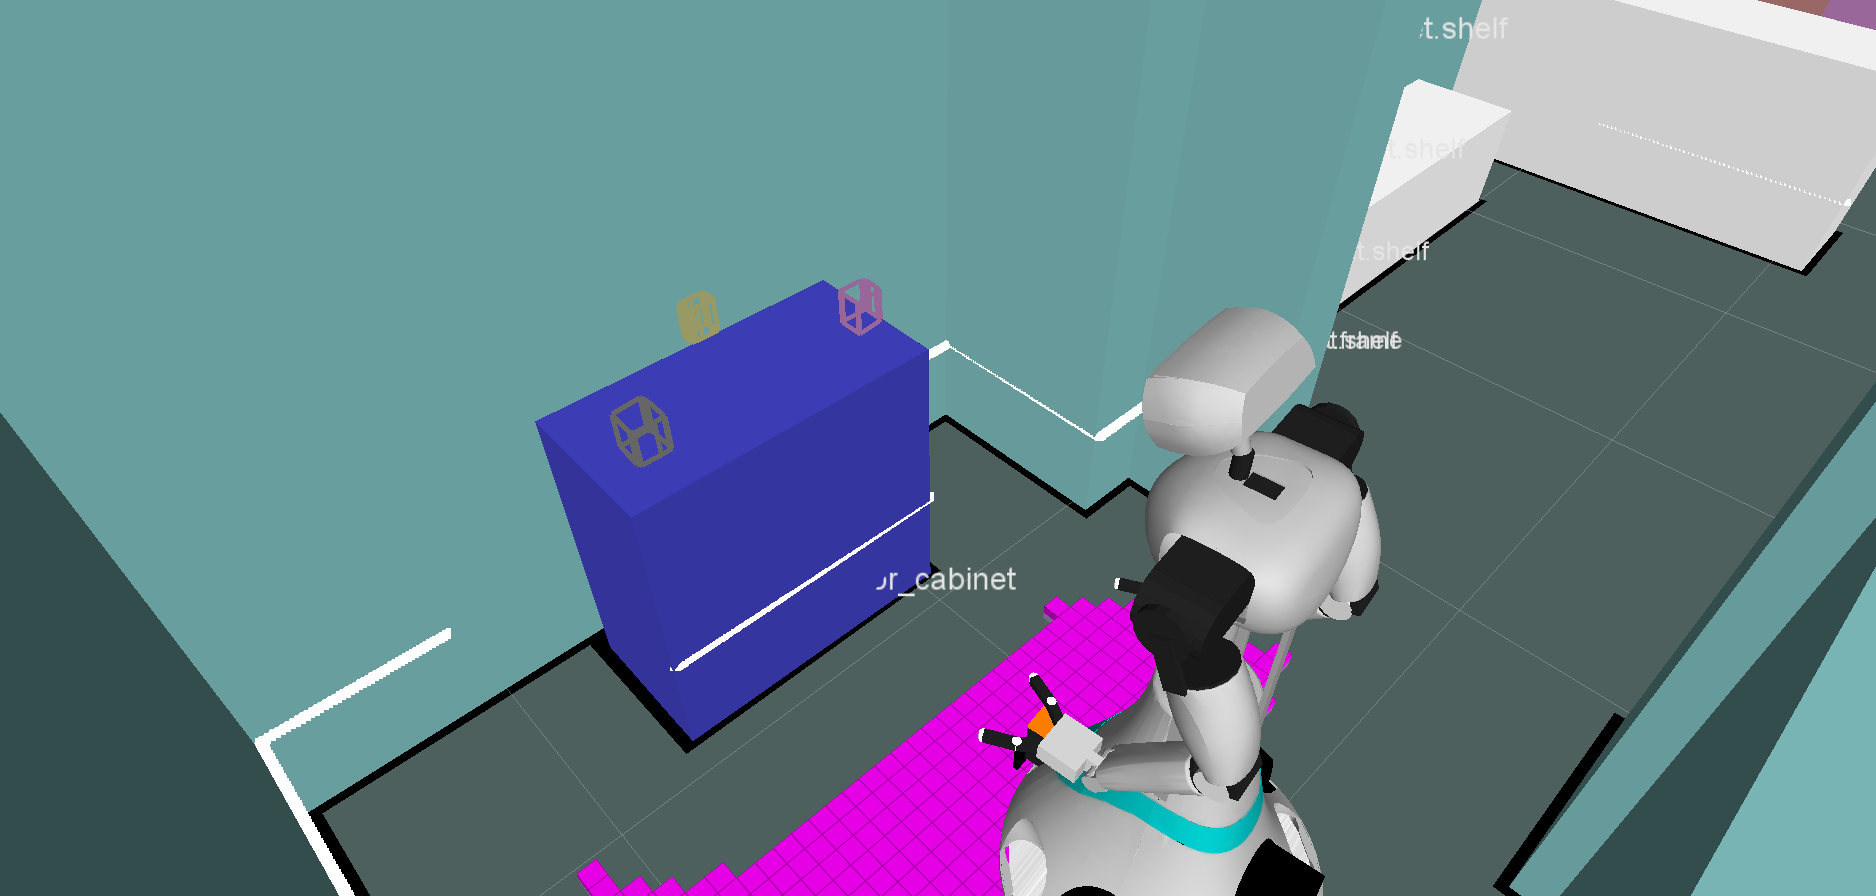
\includegraphics[width = 0.8\linewidth]{Figures/ed_segmentation}
    %\vspace{-0.5em}
	\caption{A view of the world model created with ED. The figure show the occupation grid as well as (unknown) objects recognized on top of the cabinet.}
	\label{fig:ed_segmentation}
    %\vspace{-0.5cm}
\end{figure}



%\subsection{Localization}
%The \acrshort{ed}-localization plugin\footnote{\url{https://github.com/tue-robotics/ed localization}} implements Monte Carlo localization based on the environment description in ED, laserscan readings (sensor\_msgs/Laserscan) and a valid transformation between the /odom and the /base\_link frame of the robot (tf). It does not differ much from the ROS AMCL package\footnote{\url{http://wiki.ros.org/amcl}}; where the AMCL package uses a grid map as representation, the ED-localization plugin uses a 2D render from its world model. 
Slam\_gmapping\footnote{\url{http://wiki.ros.org/gmapping}} - ROS simultaneous localization and mapping (SLAM) component - was configured for usage on PR2 and Toad robots. It requires only laser scanner (messages of type sensor\_msgs/LaserScan) and odometry (TF transform between robot base and odometry reference frame). When there is a static environment as in the use case it can be used to obtain 2D map and then robot can localize against this map by the \acrshort{amcl} package. The \acrshort{amcl} also requires only laser scanner and odometry and provides reasonably robust localization. Full description of both components is given on their respective \acrshort{ros} wiki pages.

\subsection{Localization, Navigation and Exploration}
The \href{{https://github.com/tue-robotics/ed_localization}}{\acrshort{ed}-localization plugin} implements \acrshort{amcl} based on a 2D render from its world model.

%In order to navigate, a model of the environment is required. This model is stored in the (\acrshort{ed}). From this model, a planning representation is derived that enables using the model of the environment for navigation purposes.
%\begin{figure}[hb]
%    %\vspace{-0.3cm}
%	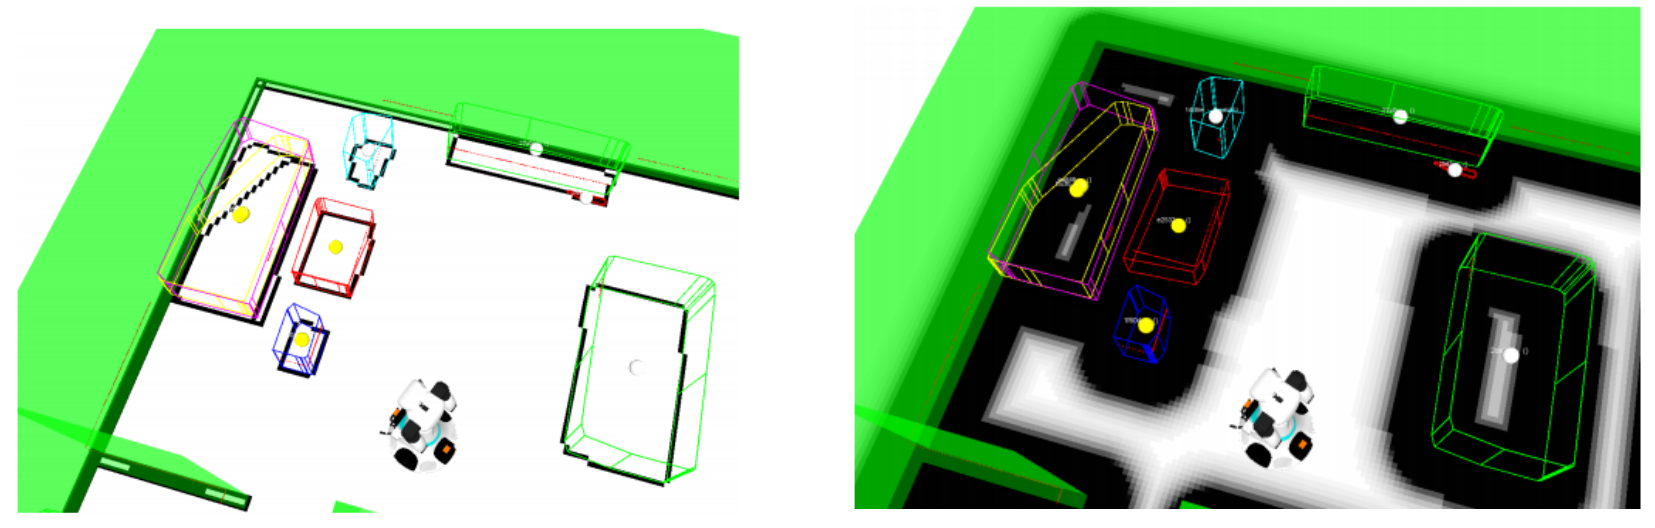
\includegraphics[width = \linewidth]{Figures/ed_navigation}
%    %\vspace{-1em}
%	\caption{Grid representation of the environment.}
%	\label{fig:ed_navigation}
%    %\vspace{-0.2cm}
%\end{figure}
With use of the \href{https://github.com/tue-robotics/ed_navigation}{ed\_navigation plugin}, an occupancy grid is derived from the world model and published as a nav\_msgs/OccupancyGrid. This grid can be used by a motion planner to perform searches in the configuration space of the robot.
\\
With the use of the \href{https://github.com/tue-robotics/cb_base_navigation}{cb\_base\_navigation} ROS package. The robots are able to deal with end goal constraints. With use of a ROS service, provided by the ed\_navigation plugin, an end goal constraint can be constructed w.r.t. a specific world model entity described by ED. This enables the robot to not only navigate to poses but also to areas or entities in the scene, as illustrated by Figure \ref{fig:ed_navigation_constraints}.
\begin{figure}[h]
    \centering
    %\vspace{-0.2cm}
	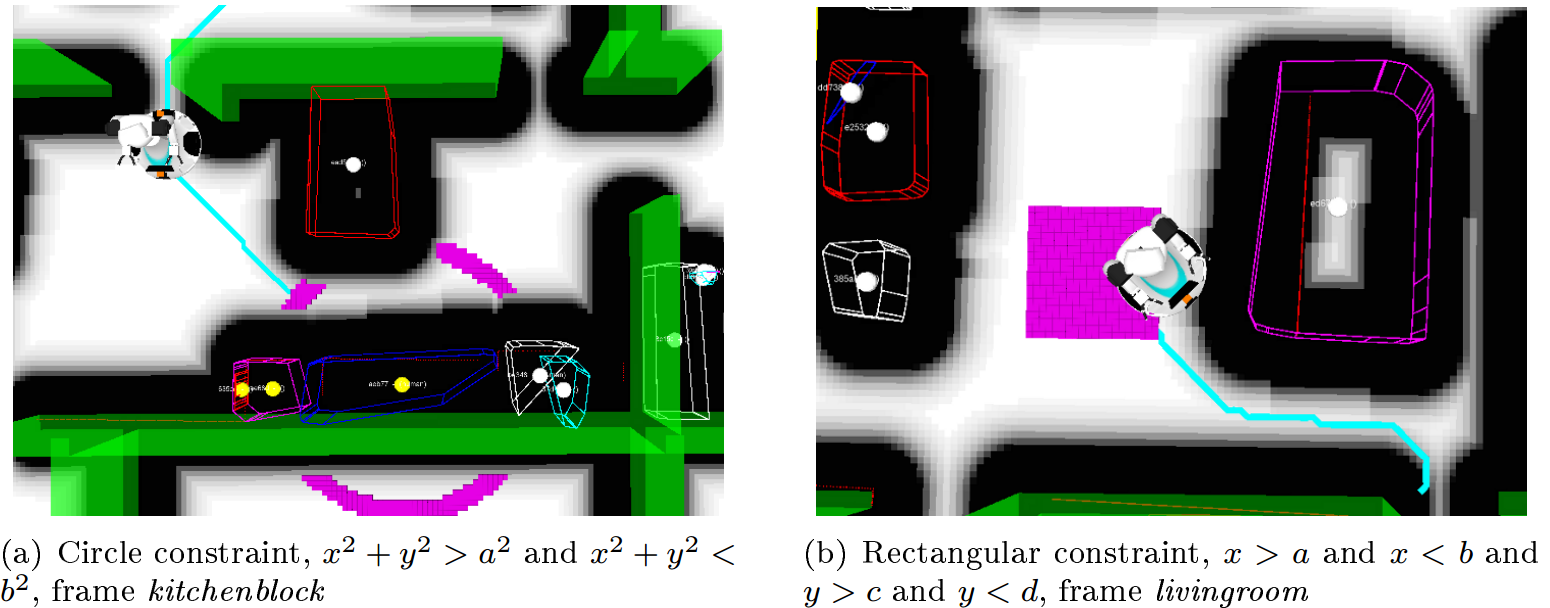
\includegraphics[width = 0.9\linewidth]{Figures/ed_navigation_constraints}
    %\vspace{-0.5em}
	\caption{Navigation position constraints w.r.t. other entities in the environment}
	\label{fig:ed_navigation_constraints}
    %\vspace{-0.5cm}
\end{figure}
Somewhat modified versions of the local and global ROS planners available within move\_base are used. \\The configurations for move\_base node has now been created for the AMIGO and SERGIO robots, the HSR node will be added. The node integrates local and global path planning and local control. Its actionlib interface has become in fact standard for sending 2D navigation goals to robots in ROS. 

\subsection{Object detection and recognition}
\subsubsection{Detection \& Segmentation}
ED enables integrating sensor data with use of the plugins present in the ed\_sensor\_integration package. Two different plugins do exist:
1. laser\_plugin: Enables tracking of 2D laser clusters. This plugin can be used to track dynamic obstacles such as humans.
2. kinect\_plugin: Enables world model updates with use of Kinect data. This plugin exposes several ROS services that realize different functionalities:
a. Segment: Service that segment sensor data that is not associated with other world model entities. Segmentation areas can be specified per entity in the scene. This allows to segment object ‘on-top-of’ or ‘in’ a cabinet.
b. FitModel: Service that fits the specified model in the sensor data of the Kinect. This allows updating semi-static obstacles such as tables and chairs.
\\
The ed\_sensor\_integration plugins enable updating and creating entities. However, new entities are classified as unknown entities.
\begin{figure}[h]
    \centering
    %\vspace{-0.3cm}
	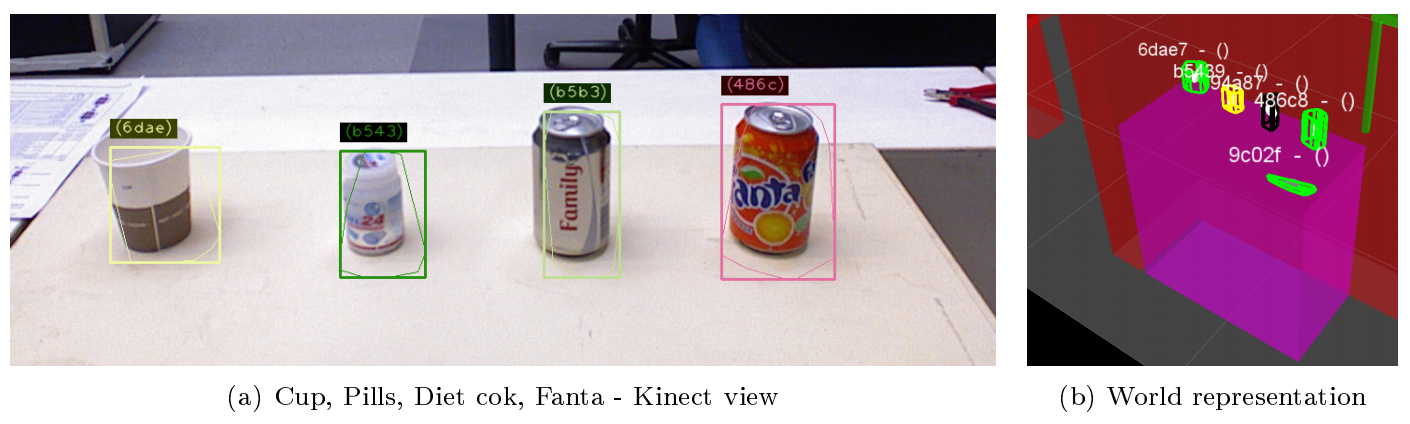
\includegraphics[width = 0.9\linewidth]{Figures/ed_perception}
    %\vspace{-1em}
    \caption{}
	\label{fig:ed_perception}
    %\vspace{-0.5cm}
\end{figure}

\subsubsection{Recognition using Deep Learning}
In order the classify or train unknown entities, the \href{https://github.com/tue-robotics/ed_perception}{ed\_perception plugin} exposes ROS Services to classify the entities in the world model. The ed\_perception module interfaces with various image\_recognition nodes that apply state of the art image classification techniques based on \acrfull{cnn} \ref{fig:cnn}.
\begin{figure}[h]
    \centering
    %\vspace{-0.3cm}
	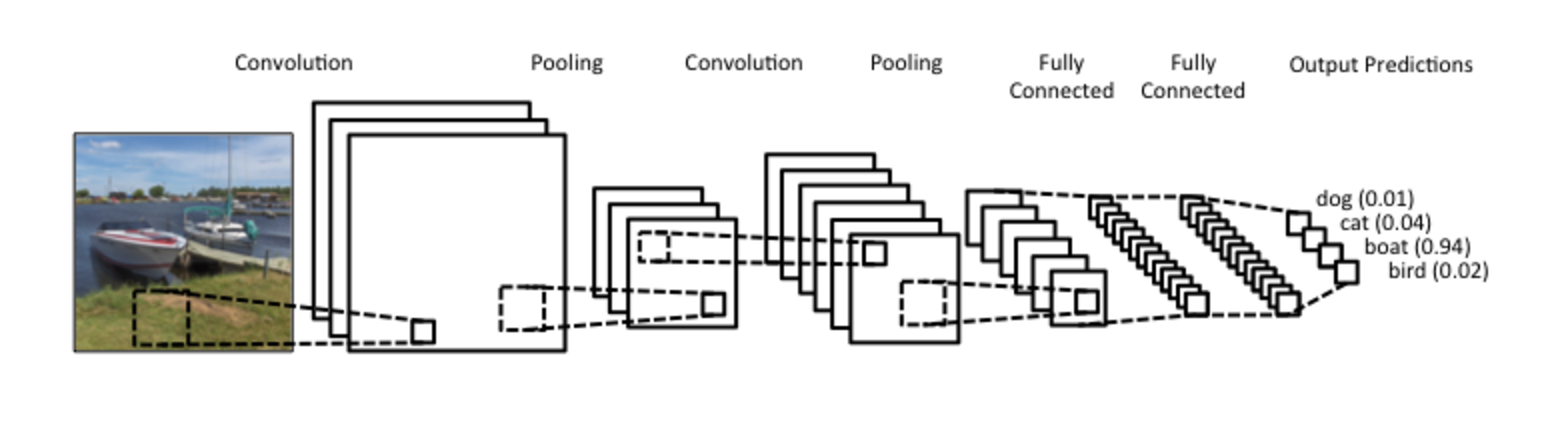
\includegraphics[width = 0.9\linewidth]{Figures/cnn}
    %\vspace{-1em}
    \caption{}
	\label{fig:cnn}
    %\vspace{-0.5cm}
\end{figure}
Object recognition is done using Tensorflow: retraining the top-layer of a Inception V3 neural network. The top layers are retrained on a custom dataset using a soft-max top-layer that maps the image representation on a specified set of labels.
\\
Face detection and recognition is done using Openface based on Torch. Openface is an existing state-of-the-art face recognition library. We implemented a ROS node that enables the use of these advanced technologies within the ROS network.
\\
In order to create a new training set for specific objects, the ed\_perception and the image\_recognition packages contains several tools for segmenting and annotating object. Also tools for retraining neural networks are included.
\\
Our image recognition ROS packages can be found at \href{https://github.com/tue-robotics/image_recognition}{GitHub} with tutorials and documentation. 

\subsection{Object grasping, moving and placing}
As for manipulating objects, the architecture is only focused on grasping. The input is the specific target entity in the world model (ED). The output is the grasp motion, i.e. joint positions for all joints in the kinematic chain over time. Figure \ref{fig:grasping_pipeline} shows the grasping pipeline.
\begin{figure}[ht]
	\includegraphics[width = \linewidth]{Figures/grasping_pipeline}
	\caption{Grasping pipeline.}
	\label{fig:grasping_pipeline}
\end{figure}
A python executive queries the current pose of the entity from \acrshort{ed}. The resulting grasp pose goes to the grasp precompute component which makes sure that we approach the object in a proper way. Finally, MoveIt will solve the IK solution and produces joint trajectories over time with use of the current configuration, the URDF model and the final configuration. Note that MoveIt currently does not take any information from \acrshort{ed} into account. Finally, the trajectories are sent to the reference interpolator which sends the trajectories either to the controllers or the simulated robot. 

\subsection{Reasoning}
The reasoning layer of the AMIGO ROS based software consists of a set of finite state machines (robot\_smach\_states1) that build upon the robot’s skill layer (robot\_skills2). These state machines are useful if you want the robot to execute some complex plan, where all possible states and state transitions can be described explicitly. 
The implementation is done with use of the open-source SMACH3 package. SMACH is a task-level architecture for rapidly creating complex robot behaviours. At its core, SMACH is a ROS-independent Python library to build hierarchical state machines. SMACH is a new library that takes advantage of very old concepts in order to quickly create robust robot behaviour with maintainable and modular code.

\subsection{Human-Robot Interface}
\subsection*{Overview}

In order to interact with the robot aside of speech, a web-based Graphical User Interface (GUI) has been designed. An HTML5 website \footnote{\texttt{https://github.com/tue-robotics/tue\_mobile\_ui}} is hosted on the robotic platform that offers a GUI to multiple users on different platforms with use of a Robot API\footnote{\texttt{https://github.com/tue-robotics/robot-api}} implemented in Javascript. Figure \ref{fig:webgui_architecture} shows an overview of how the user can interact with the robot via this interface.

\begin{figure}[ht]
        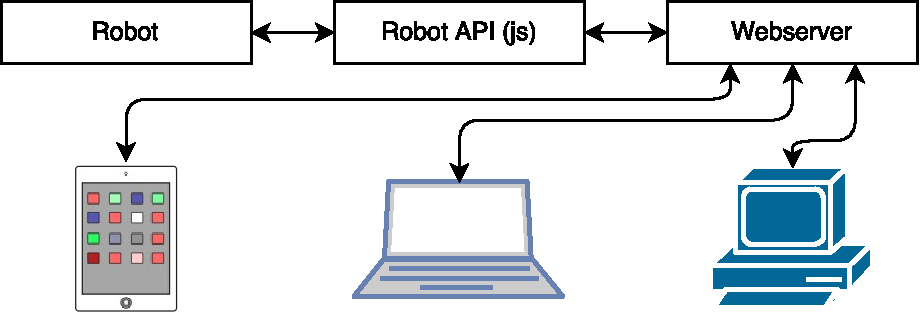
\includegraphics[width = \linewidth]{webgui_architecture}
        \caption{Overview webGUI architecture. The robot's functionalities are exposed with use of the Robot API that is implemented in javascript. The Webserver that is hosting the GUI connects this Robot API to a graphical user interface that is offered to multiple clients on different platforms.}
        \label{fig:webgui_architecture}
\end{figure}

\subsection*{Illustration}




%\newpage
\section{List of externally available components that are planned to be implemented}
An overview of the software used by the Tech United Eindhoven @Home robots can be found in Table~\ref{tab:softwarespec}.
All our software is developed open-source at GitHub\footnote{\texttt{https://github.com/tue-robotics}}

\begin{table}[H]
    \begin{center}
    \caption{Software overview of the robots.}
    \label{tab:softwarespec}
    \vspace{-0.1cm}
    \renewcommand{\arraystretch}{1.0}
    \setlength{\tabcolsep}{5pt}
        \begin{tabular}{p{0.3\textwidth} p{0.7\textwidth}}
        	\toprule
            Operating system & Ubuntu 14.04 LTS Server\\

            Middleware & ROS Indigo~\cite{Quigley2009}\\

            Low-level software & Orocos Real-Time Toolkit~\cite{Bruyninckx2001}\\

            World model & \acrfull{ed}, custom \newline \url{https://github.com/tue-robotics/ed}\\

            Localization & Monte Carlo~\cite{Fox2003} using \gls{ed}, custom \newline \url{https://github.com/tue-robotics/ed_localization}\\

            SLAM & Gmapping: \texttt{http://wiki.ros.org/gmapping}\\

            Navigation & Global: custom A* planner\newline Local: modified ROS DWA~\cite{Fox1997}\\

            Arm navigation & Custom implementation using MoveIt and Orocos KDL\\

            Object recognition & Tensorflow ROS \newline \url{https://github.com/tue-robotics/image_recognition/tree/master/tensorflow_ros} \\

            People detection & Custom implementation using contour matching \\
            Face detection \& recognition & Openface ROS \newline \url{https://github.com/tue-robotics/image_recognition/tree/master/openface_ros} \\
            Speech recognition & Dragonfly + Windows Speech Recognition \newline \texttt{http://code.google.com/p/dragonfly/}\\
            Speech synthesis & Philips Text-to-Speech\\
            Task executors & SMACH\newline\texttt{http://wiki.ros.org/smach}\\
            \bottomrule
        \end{tabular}
    \end{center}
\end{table}


\subsection{Focus of research and scientific contributions}
Halve A4

\subsection{Re-usability of the system for other research groups}
All of our software is open-source designed. Our repositories are available on GitHub, https://github.com/tue-robotics. All packages are equipped with documentation and tutorials. In example, our ROS wrapper for openface is forked by the Toyota Research Institute.
Nog iets verder uitbreiden

\subsection{Applicability of the approach in the real world}
For us, science doesn’t stop at software simulation. At TUE, our test infrastructure contains real life environments. Here, different room types can be simulated (i.e. home, care institution) and real life products are used. In addition, Tech United carries out many demonstrations per year at different indoor locations throughout the Netherlands. This ensures that our concepts keep being tested. At this point our system are able to operate in dynamic environments used by humans. 

\subsection{Community Outreach and Media}
The Tech United team carries out many promotional activities to promote technology and innovation with children. These activities are carried out by separate teams of student assistants. Tech United often visits primary and secondary schools, public events, trade fairs and have regular TV performances. In 2015 and 2016 together, 100+ demos were given and an estimated 50k were reached through live interaction.
Tech United has also got a very active (\href{www.techunited.nl}{website}, and interacts on many social media mediums: \href{https://www.facebook.com/techunited}{Facebook}, \href{https://www.youtube.com/user/TechUnited}{YouTube}, \href{https://twitter.com/TechUnited}{Twitter} and \href{https://www.flickr.com/photos/techunited/}{Flickr}. Our robotics videos are often shared on the IEEE video Friday website.


%\bibliographystyle{unsrt}
%\bibliography{refs}


\end{document} 